\documentclass{abnt}
\usepackage[utf8]{inputenc}
\usepackage[num]{abntcite}
\usepackage{graphicx}
\usepackage{url}
\usepackage{caption}
\usepackage{listings}
\usepackage[brazil]{babel}
\addto\captionsbrazil{%
\def\bibname{References}%
\def\abstract{Abstract}
}

\lstset{
basicstyle=\small\sffamily,
numbers=left,
numberstyle=\tiny,
frame=tb,
columns=fullflexible,
showstringspaces=false
}

\graphicspath{{imagens/}}

\begin{document}
\autor{André Taiar Marinho Oliveira}

\titulo{A look into new programming languages}

\orientador[Orientador:\\]{Prof. Dr. Fernando Magno Quintão Pereira}

\comentario{Apresentado como requisito da disciplina de Monografia em Sistemas de Informação do DCC/UFMG}

\instituicao{Universidade Federal de Minas Gerais \par Instituto de Ciências
Exatas \par Departamento de Ciência da Computação}

\local{Belo Horizonte} \data{2015/2}

\capa
\folhaderosto

\begin{resumo}
There are hundred of programming languages out there. Which one should we use?
Which help do we have to choose well? How do they compare to each other? This
document is an attempt to provide some answers to these questions. Naturally, it
would not be possible to provide complete answers: as I mentioned, there are too
many programming languages. Nevertheless, we chose four languages with a
potential to grow in importance in the coming years. These programming languages
are Ceylon, Dart, Elixir and Rust. During this project, we shall be
talking about each one of them. These discussions will be in breath, not in
depth. Their goal is to provide the reader with the minimum of information
necessary to compare them, and who knows, to lure one or other interested person
in learning them in a greater level of details. In any case, we hope to
contribute a bit to the popularization of these programming languages, which -
likely - will be paramount to the development of computer science in the next
ten years.\\


\textbf{Keywords}: programming languages, ceylon, dart, elixir, rust.
\end{resumo}

\sumario %comando que gera o sumário automaticamente
\listoffigures %comando que gera um sumário para a lista de figuras do texto automaticamente


% \begin{figure}[!htb]
% 	\centering
% 	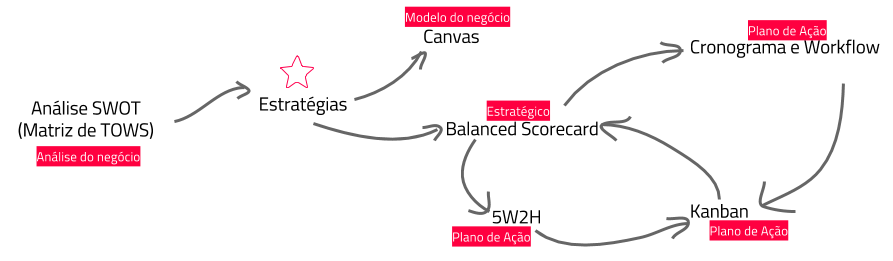
\includegraphics[width=\textwidth]{fluxograma_exemplo.pdf}
% 	\caption{Exemplo de fluxo de trabalho possível no sistema}
% 	\label{Rotulo}
% \end{figure}

\chapter{Ceylon}
\section{Ceylon language introduction}
\subsection{How did it appear?}

Red Hat\cite{1_1} is the world's leading provider of open source software
solutions and it has initiated and sponsored\cite{1_2} the development
of the Ceylon programming language. Ceylon is first and foremost an open source
community project.

According to the language's F.A.Q\cite{1_3}, Ceylon was designed to be a
modern Java with better specification, as we can see in the excerpt:

\begin{quote}
Well, we've been designing and building frameworks and libraries for Java for
ten years, and we know its limitations intimately. And we're frustrated. The
most recent releases of Java go some distance to alleviating some problems,
but even the newest language features strain to accommodate past mistakes and
the requirement for full backward compatibility.
But much of our frustration is not even with the Java language itself. The
extremely outdated class libraries that form the Java SE SDK are riddled with
problems. Developing a great SDK is a top priority of the project.
\end{quote}

\subsection{Why was it designed and implemented?}

Ceylon has a lot of interesting features but, we can start with this
definition on the homepage\cite{1_4}: \textit{"Ceylon is a language for writing
large programs in teams"}. The language is deeply influenced by Java and it was
designed and implemented by people who were hugely involved with Java. People
like Gavin King, the lead of the Ceylon project in Red Hat and also the creator
of Hibernate\cite{1_5} (the most popular Object Relational Mapper for Java) and
other projects in the Oracle's platform.

Modularity is in the very core of the Ceylon language. When a Ceylon's code is
compiled, it produces module archives. In fact is very similar to Java's
modules. It generates a *.car file, with *.class files zipped on it. Just
like Java's *.jar. You'll never be exposed to unpacked *.class files in
Ceylon. So here we got 2 conclusions. The first one is that the compiler
really forces the modularity and facilitates the distribution of the generated
code. The second one is that the Ceylon compiled code runs on the Java Virtual
Machine (JVM). This second fact is very important because by running on the JVM,
Ceylon's code is fully interoperable with Java, the Java SDK and its libraries.
In fact, this interoperability is a major priority of the project.

This is an example of the use of the Java's HashMap data structure on a Ceylon
program:

\begin{lstlisting}[label=cujhm,caption=Ceylon using Java HashMap]
import java.util { HashMap }

value javaHashMap = HashMap<String,Integer>();
javaHashMap.put("zero", 0);
javaHashMap.put("one", 1);
javaHashMap.put("two", 2);
print(javaHashMap.values());
\end{lstlisting}

Ceylon runs on the JavaScript virtual machine too. In fact the Ceylon's compiler
can generate JavaScript code if told to do so. It generates modular JavaScript
in the CommonJS modules format. We'll see more on JavaScript generation in the
future.

\begin{lstlisting}[label=cjs,caption=Ceylon JavaScript]
dynamic {
    dynamic req = XMLHttpRequest();
    req.onreadystatechange = void () {
        if (req.readyState==4) {
            document.getElementById("greeting")
                    .innerHTML = req.status==200
                            then req.responseText
                            else "error";
        }
    };
    req.open("GET", "/sayHello", true);
    req.send();
}
\end{lstlisting}

Ceylon's project always tells how important is the toolset for a complete and
successful programing project so it ships with a really great Integrated
Development Environment (IDE) built on a Eclipse plug-in. We'll see more
detailed information on the {install and run} section below.

\subsection{How can we use it, e.g., install and run?}

By running in the JVM, the Ceylon's compiler got the advantage to run
on every operating system which has a Java Virtual Machine implementation. It  
runs both on Java 7 and Java 8 (prior versions are not supported). So before
installing the Ceylon package, be sure to have the correct Java version
installed. On this work, I'm using the 1.1 version of the language, released on
09 October 2014.

For installation on a Mac, you can use the Homebrew installer:

\begin{verbatim}
$ brew update
$ brew install ceylon
\end{verbatim}

There are packages for both Debian and Fedora/Red Hat GNU/Linux flavors on the
project's download page\cite{1_10}.

For a platform agnostic installation, download the zip archive
(\url{http://ceylon-lang.org/download/dist/1_1_0}),
unzip on your system's prefered folder and add the \textbf{/ceylon-1.1.0/bin}
folder to the path of your system. In a unix-like system you can do that by
adding the line below on the \textbf{~/.bashrc} file of you user's directory:

\begin{verbatim}
$ export PATH="/path/to/ceylon-1.1.0/bin:$PATH"
\end{verbatim}

Now let's check if the installation works. By forcing the modularity, Ceylon
implies some conventions on the compilation process. At first the code we'll
write must be on a \textbf{"source"} directory. So place the following code on a
file called \textbf{"./source/hello.ceylon"}:

\begin{lstlisting}[label=hello,caption=Ceylon Hello World]
shared void hello() {
  print("Hello Ceylon!");
}
\end{lstlisting}

Outside the \textbf{source's} folder, run the command:

\begin{verbatim}
$ ceylon compile source/hello.ceylon
\end{verbatim}

Checkout the \textbf{module} folder created on the same level as the 
\textbf{source} folder. Check it's content for the \textit{*.car} file and some
others. To run the compiled source, run the following command:

\begin{verbatim}
$ ceylon run --run hello default
\end{verbatim}

\subsection{Simple programs}

I will demonstrate some features of the language by writing some simple programs
and analyzing some points right after it.

\subsubsection{The treelike structure, simple classes and visibility}

I'll use this example to illustrate the treelike structure that Ceylon has.
Ceylon's named argument lists provide an elegant way for initializing objects
and collections. The goal of this facility is to replace the use of XML for
expressing hierarchical structures such as documents, user interfaces,
configuration and serialized data.

I'll use this notation to create a binary search tree and make a depth-first
in-order traversal.

\begin{lstlisting}[label=ctls,caption=Ceylon treelike structure]
shared class Node(val, left = null, right = null) {
	shared Integer val;
	shared Node? left;
	shared Node? right;
}

shared void caminhamento_central(Node b) {
	if(exists next = b.left) {
		caminhamento_central(next);
	}
	process.write(b.val.string + " ");
	if(exists next = b.right) {
		caminhamento_central(next);
	}
}

shared void run() {
	Node arvore = Node {
		val = 1;
		left = Node {
			val = 2;
			left = Node {
				val = 4;
				left = Node { val = 8; };
				right = Node { val = 9; };
			};
			right = Node {
				val = 5;
				left = Node { val = 10; };
				right = Node { val = 11; };
			};
		};
		right = Node {
			val = 3;
			left = Node {
				val = 6;
				left = Node { val = 12; };
				right = Node { val = 13; };
			};
			right = Node {
				val = 7;
				left = Node { val = 17; };
				right = Node { val = 15; };
			};
		};
	};

	caminhamento_central(arvore);
	print("");
}
\end{lstlisting}

The result of this program must be:

\begin{verbatim}
8 4 9 2 10 5 11 1 12 6 13 3 17 7 15
\end{verbatim}


Look at the word \textit{shared} on some points of the example. This \textit{shared}
annotation marks a declaration as being visible outside the scope in which it is
defined, or a package as being visible outside the module to which it
belongs\cite{1_6}.

It's all about visibility\cite{1_7}. Classes, interfaces, functions, values,
aliases, and type parameters have names. Occurrence of a name in code implies a
hard dependency from the code in which the name occurs to the schema of the
named declaration. We say that a class, interface, value, function, alias, or
type parameter is visible to a certain program element if its name may occur in
the  code that belongs to that program element. The visibility of a declaration
depends upon where it occurs, and upon whether it is annotated \textit{shared}. 

\subsubsection{Random numbers and Java interoperability}

Ceylon's SDK is under constant development\cite{1_8} and there aren't a random
numbers implementation yet. But Ceylon can use the Java SDK, so I'll use the
Java random numbers interface to work on a Ceylon's simple example.

\begin{lstlisting}[label=w1,caption=Random number from Java]
// Import from Java SDK
import java.util { Random }

shared Integer getRandomInteger(Integer a, Integer b, Random r) {
	value range = b - a + 1;
	value fraction = (range * r.nextDouble());
	return (fraction + a).integer;
}

shared void run() {
    Random random = Random();
    for(number in 1..100) {
        print(getRandomInteger(1, 100, random));
    }
}
\end{lstlisting}

To use the Java SDK (and other libraries from outside the language's SDK) you
must use the module structure that is conventioned in the language. I'll use
this example to show it.

Save the code above on a file called \textbf{random.ceylon} inside of the
following structure of directories: \textbf{./source/example/random/}. This
structure corresponds to the namespace of the module we are creating. It's just
like Java always did.

Inside this same folder, create the file \textbf{module.ceylon}. It is the file
that will specify the dependencies our module have with external resources (like
Java libraries) and formalize it's namespace. The content of this file must be:

\begin{lstlisting}
module example.random "1.0.0" {
    import java.base "8";
}
\end{lstlisting}

The \textit{java.base} module in JDK has Java base packages such as
\textit{java.lang}, \textit{java.util}, \textit{java.io}, \textit{java.net},
\textit {java.text}, NIO and security\cite{1_9}. All done, inside of the
project's root, run the command:

\begin{verbatim}
$ ceylon compile
\end{verbatim}

The module will be compiled with the correct dependencies and the files will be
generated in the correspondent directory of the module (in our example, it
would be $./modules/example/random/1.0.0/$). Then we can run the code
with the command:

\begin{verbatim}
$ ceylon run example.random
\end{verbatim}

The program will execute calling the method \textit{run} (like the \textit{main}
method in Java) inside the package \textit{example.random}.
\section{Ceylon language usage}

To show some more interesting features of Ceylon, I wrote a version of the
Producer-consumer problem. This is a classic example of a multi-process
synchronization problem. It describes two processes, the producer and the
consumer, who share a common, fixed-size storage (buffer) used as a queue. The
producer's job is to generate a piece of data, put it into the storage and start
again. At the same time, the consumer is consuming the data (i.e., removing it
from the storage) one piece at a time. The problem is to make sure that the
producer won't try to add data into the storage if it's full and that the
consumer won't try to remove data from an empty storage\cite{2_1}.

The implementation relies strongly of the Java Thread libraries. The Producer
and the Consumer objects runs on different threads, each instance of each
object. The Storage class manage the additions of the producers and the
remotion of the consumers on the buffer. For synchronization I used the Java's
Semaphore class.

Let's see the code and I'll give the explanations:

\begin{lstlisting}[label=cpc,caption=Ceylon Producer-Consumer example]
import ceylon.collection { ArrayList }
import java.util.concurrent { Semaphore }
import java.lang { Thread, Math }

shared Integer getRandomInteger(Integer a, Integer b) {
	value range = b - a + 1;
	value fraction = (range * Math.random());
	return (fraction + a).integer;
}

class Producer(Storage storage, shared actual Integer id) extends Thread() {

	void produce() {
		if(Math.random() < 0.5) {
			storage.add(this);
		}
	}

	shared actual void run() {
		while(true) {
			this.produce();
			this.sleep(getRandomInteger(1, 4) * 1000);
		}
	}

}

class Consumer(Storage storage, shared actual Integer id) extends Thread() {

	void consume() {
		if(Math.random()  < 0.5) {
			storage.get(this);
		}
	}

	shared actual void run() {
		while(true) {
			this.consume();
			this.sleep(getRandomInteger(1, 4) * 1000);
		}
	}

}

class Storage(shared Integer storageSpaces) {

	value buffer = ArrayList<Integer>(storageSpaces);
	variable Integer lastEmpty = 0;
	value m = Semaphore(1);

	for(i in 0..(this.storageSpaces - 1)) {
		this.buffer.push(0);
	}

	shared void get(Producer|Consumer actor) {
		m.acquire();
		assert(actor is Consumer);
		print("[Consumer " + actor.id.string + "] Wants to consume!");
		if(this.lastEmpty == 0) {
			print("[Storage] I have nothing for you now. Look: ");
		} else {
			this.lastEmpty--;
			this.buffer.set(this.lastEmpty, 0);
			print("[Storage] Ok, I got a thing for you.");
		}
		m.release();
		this.printBuffer();
	}

	shared void add(Producer|Consumer actor) {
		m.acquire();
		assert(actor is Producer);
		print("[Producer " + actor.id.string + "] Produced something.");
		if(this.lastEmpty == this.storageSpaces) {
			print("[Storage] I'm full! Can't take it right now, look:");
		} else {
			this.buffer.set(this.lastEmpty, 1);
			this.lastEmpty++;
			print("[Storage] Tank you! I'll store it.");
		}
		m.release();
		this.printBuffer();
	}

	shared void printBuffer() {
		m.acquire();
		process.write("[ ");
		for (load in this.buffer) {
			process.write(load.string + " ");
		}
		print("]");
		m.release();
	}

}

shared void run() {
	value storage = Storage(15);

	value p1 = Producer(storage, 1);
	value p2 = Producer(storage, 2);

	value c1 = Consumer(storage, 1);
	value c2 = Consumer(storage, 2);

	p1.start();
	p2.start();

	c1.start();
	c2.start();
}
\end{lstlisting}

The first thing we see are the imports. We are already used to them, in the
first article where I used already some Java interoperability and explained the
concept of modules. Every of these things are used here.

\subsection{Toplevel functions}

After that, we can see a function called \textit{getRandomInteger}. In Ceylon, this is a
\textit{toplevel function}. A toplevel function declaration, or a function declaration
nested inside the body of a containing class or interface, may be annotated
\textit{shared} (in the last article, I talked about the shared annotation and the
visibility issues). A toplevel shared function is visible wherever the package
that contains it is visible.

Another interesting thing about \textit{toplevel} functions in Ceylon is that they can
be called by external programs on the system. On the example, I'll modify the
function a little so we can see what is going on:

\begin{lstlisting}[label=cri,caption=Ceylon random integer function]
shared Integer getRandomInteger(Integer a = 1, Integer b = 5) {
	value range = b - a + 1;
	value fraction = (range * Math.random());
	value gen = (fraction + a).integer;
	print(gen);
	return gen;
}
\end{lstlisting}


The toplevel function must have no parameters (or default value parameters) so
you can call her externally. By placing our program inside a module called
\textit{prodcons} (see the module session on the first article), we can compile
and run the program like:

\begin{verbatim}
$ ceylon compile
$ ceylon run --run prodcons::getRandomInteger prodcons
\end{verbatim}

The random integer numbers between $[1, 5[$ will be generated by the program and
printed on the screen.

\subsection{Classes}

We have then, the class \textit{Producer} which is the very same class of the
\textit{Consumer}, except it calls different methods of the \textit{Storage} class. The
first interesting thing we can see is that Ceylon 1.1 has no constructor
methods. Since the earliest versions of the language, it supports a streamlined
syntax for class initialization where the parameters of a class are listed right
after the class name, and initialization logic goes directly in the body of the
class\cite{2_2}.

We can instantiate the class Producer like this:

\begin{lstlisting}[label=cpc,caption=Ceylon Producer-Consumer example]
value prod = Producer(Storage(15), 1);
\end{lstlisting}

The ability to refer to parameters of the class directly from the members of the
class has the intuit to cut down on verbosity. However, there are moments when
we would really appreciate the ability to write a class with multiple
initialization paths, something like constructors in Java. The constructors are
being implemented on Ceylon and will be available in the next versions of the
language.

The annotation \textit{shared} on the parameter \textbf{id} says that this is like a Java's
\textit{public} member of the class. \textbf{storage} is not annotated, so it is like a
private one.

Look at the annotation \textit{actual} that is used in the same \textbf{id} parameter and in
the \textbf{run} method. It tells that, inside the inheritance tree of possible
values (since the two classes extends the Thread Java class) that could
overwrite the method or the variable, this is the very one that will do it. So,
\textbf{shared id} is overwriting the parameter id (probably on the Thread Java
class) and \textbf{shared run} is overwriting a run method (surely on the Thread Java
class). In the case of Interfaces, the word to tell that a class implements
(from Java) an interface is \textbf{satisfies}; so a class \textbf{satisfies} an
interface. The annotation \textbf{actual} is used to tell what method is
\textbf{satisfying} the Interface's specification.

\subsection{Collections, sequences and tuples}

Ceylon SDK has a great library that implements every kind of collections, just
like Java does. There are interfaces and classes to implement all sort of
operations involving \textit{ArrayList}, \textit{LinkedList}, 
\textit{PriorityQueue}, \textit{HashSet}, \textit{HashMap}, \textit{TreeSet},
\textit{TreeMap} etc\cite{2_3}. In our example, I used an \textit{ArrayList}
(which is the implementation of a list using arrays) to store the production of
the Producer.

In the example, I used a loop to initialize every cell of the \textit{buffer}
list with the value zero. In the for loop, I used a \textbf{Sequence} to
generate the iterable value. Sequence is a type that in the first time could
look very familiar to a Java array but in fact they are very different. First of
all, the sequence is a \textbf{immutable} type and not a mutable concrete type
like the array. We can't set the value of an element like:

\begin{lstlisting}[label=cpc,caption=Ceylon Producer-Consumer example]
String[] operators = .... ;
operators[0] = "^"; //compile error
\end{lstlisting}

This following code, doesn't compile too:

\begin{lstlisting}[label=cpc,caption=Ceylon Producer-Consumer example]
for (i in 0..operators.size-1) {
    String op = operators[i]; //compile error
    // ...
}
\end{lstlisting}

The index operation $operators[i]$ returns an optional type \textit{String?},
which cannot be assigned to the type \textit{String}. Instead, if we need access
to the index, we use the special form of \textbf{for}:

\begin{lstlisting}[label=cpc,caption=Ceylon Producer-Consumer example]
for (i -> op in operators.indexed) {
    // ...
}
\end{lstlisting}

Ceylon has the \textbf{tuple} type too. It might be a very common use for the
most of those who already worked with a language that has tuples.

\begin{lstlisting}[label=cpc,caption=Ceylon Producer-Consumer example]
[Float,Float,String] point = [0.0, 0.0, "origin"];
\end{lstlisting}

\subsection{Type system}

Every value in a Ceylon program is an instance of a type that can be expressed
within the Ceylon language as a class. The language does not define any
primitive or compound types that cannot, in principle, be expressed within the
language itself.

Each class declaration defines a type. However, not all types are classes. It is
often advantageous to write generic code that abstracts the concrete class of a
value. This technique is called polymorphism. Ceylon features two different
kinds of polymorphism:

\begin{enumerate}
	\item \textbf{subtype polymorphism}, where a subtype \textit{B} inherits a supertype \textit{A}, and 
	\item \textbf{parametric polymorphism}, where a type definition \textit{A<T>} is parameterized by a generic type parameter T.
\end{enumerate}

Ceylon, like Java and many other object-oriented languages, features a single
inheritance model for classes. A class may directly inherit at most one other
class, and all classes eventually inherit, directly or indirectly, the class
\textit{Anything} defined in the module \textit{ceylon.language}, which acts as the root of
the class hierarchy.

In our example, we use a parameter of the methods \textit{add} and  \textit{get} which is
\textit{Producer|Consumer} type. This type means that, whateaver a \textit{Producer} or a
\textit{Consumer} parameter passed the this method, it'll work. The methods doesn't
need this, I place'em there just for exemplification. In Ceylon, this is called
\textbf{Union types}. For any types \textit{X} and \textit{Y}, the union, or disjunction, \textit{X|Y}, of
the types may be formed. A union type is a supertype of both of the given types
\textit{X} and \textit{Y}, and an instance of either type is an instance of the union type.

\subsection{Assertions and exceptions}

The assert statement validates a given condition, throwing an
\textit{AssertionException} if the condition is not satisfied. A distinguishing
characteristic of Ceylon is that exceptions aren't used to represent programming
errors. The Ceylon creators thinks that exceptions like \textit{NullPointerException},
\textit{ClassCastException} and \textit{IndexOutOfBoundsException} should never occur in at
runtime in a production system. They represent problems that must be fixed by
the programmer editing code, tend to hide the \"corner\" condition they represent
from someone reading the code and are much too low-level to carry any useful
information about the real problem. Because of that, Ceylon tries to encode
these \"corner\" conditions into the type system.
The compiler won't let you write:

\begin{lstlisting}[label=cpc,caption=Ceylon Producer-Consumer example]
print(process.arguments[1].uppercased);
\end{lstlisting}

This code isn't well-typed because $process.arguments[1]$ is of type
\textit{String?}, reflecting the fact that there might not be a second element in the
$list process.arguments$. Instead you're forced to at least take into
account the possibility that there are less than two arguments:

\begin{lstlisting}[label=cpc,caption=Ceylon Producer-Consumer example]
if (exists arg = process.arguments[1]) {
    print(arg.uppercased);
}
else {
    throw Exception("missing second argument");
}
\end{lstlisting}

Obviously, the code is a little bigger than the initial code we had but of
course the problem is very much clear, semantic and the readers of the code
would understand the problem behind the size of the arguments in a much clearer
way.

\subsection{Concurrency}

In our example, inside of the methods \textit{get} and \textit{add} of the \textit{Storage} class is
where we would have concurrency problems\cite{2_1}. To solve this potential
problems, the class uses synchronization implemented with semaphores. I used the
Semaphore class from Java \textit{"acquiring"} and \textit{"releasing"} the
execution flow whatever some of the Threads are updating the \textit{buffer} or
printing in the screen.

In Java is very common to use the \textit{synchronized} method annotation to tell a
Thread that this method have race conditions, and the JVM takes care of the
concurrency. To use it with Ceylon, I had to specifically put the call to the
synchronization methods because it doesn't have the annotation nor any kind of
compatibility with it.

\chapter{Dart}
\section{Dart language introduction}
\subsection{How did it appear?}

Dart is an open source script language focused in web applications and developed
by Google\cite{3_1}. It was announced at GOTO
Conference 2011 (Aarhus, Denmark)\cite{3_2} and
its first stable release, Dart 1.0, comes in November
2013\cite{3_3}.

It was designed by Lars Bak and Kasper Lund, both of them employed by Google.
Lars has contributed to the Chrome Browser project developing the V8 JavaScript
Engine\cite{3_4}, the open source JavaScript
engine that runs Google's browser and gave birth to some other big projects like
Node.js\cite{3_5}.

### Why was it designed and implemented?

In the words of Google\cite{3_6}:

> At Google we’ve written our share of web apps, and we’ve tried in many ways to
> make improvements to that development process, short of introducing a new
> language. Now we think it’s time to take that leap. We designed Dart to be
> easy to write development tools for, well-suited to modern app development,
> and capable of high-performance implementations.

But in pragmatic terms all this means that Google thinks that JavaScript is
unproductive and his proposal to improve it was to design a better language for
the browsers. Google is investing a lot of effort on both sides, JavaScript
and Dart\cite{3_7} and believes that developers
should have a choice when they build for the web. Adding a new option, such as
Dart, does not imply replacing the JavaScript already existing 
option\cite{3_8}.

Dart has its own Virtual Machine which enable the Dart programs to run on every
systems. There is also a **dar2js** compiler which makes Dart code compile to
JavaScript code and run on modern browsers. And there is the third option, the
Dartium\cite{3_9} project that brings the Dart VM
inside a Chromium Browser, so Dart can be used directly as a browser's script
language like JavaScript does at Chrome nowadays.

The Dart team isn't focused in bring Dart to Google Chrome but in compiling Dart
to JavaScript. They have decided not to integrate the Dart VM into
Chrome but to generate a better JavaScript compilation\cite{3_10}
\cite{3_11}.

### How can we use it, e.g., install and run?

Dart has it's own Virtual Machine and has easy installations on all major
systems. The current stable version of Dart is **1.12.2**. For installation on a
**Mac** you can use Homebrew:

```
brew tap dart-lang/dart
brew install dart
```

Also you can install the Dartium browser with:

```
brew tap dart-lang/dart
brew install dart --with-content-shell --with-dartium
```

For **Linux** there are **Debian** packages and these are the commands for
installation on the Debian based systems:

```
sudo apt-get install apt-transport-https
sudo sh -c 'curl https://dl-ssl.google.com/linux/linux_signing_key.pub | apt-key add -'
sudo sh -c 'curl https://storage.googleapis.com/download.dartlang.org/linux/debian/dart_stable.list > /etc/apt/sources.list.d/dart_stable.list'
sudo apt-get update
sudo apt-get install dart
```

There are other options to build and install on **various Linux** distros\cite{3_12}.

There is also the versions of the SDK where you can download the portable
package and link to your system's path whatever you want:
[https://www.dartlang.org/downloads/archive/](https://www.dartlang.org/downloads/archive/).

Now let's check if the installation works. In any path (Dart doesn't force
directory structure) create the file called _hello.dart_ with the following
content:

```dart
main() {
  print("Hello Dart!");
}
```

Run with ```dart hello.dart``` and the "Hello Dart!" message must show up. Now
test the JavaScript compilation by running, with the same _hello.dart_ file, the
command:

```
dart2js hello.dart
```

You might have the message _Dart file (hello.dart) compiled to JavaScript:
out.js_. The contents of the file _out.js_ is huge if compared to the initial
Dart code. We will have more details of JavaScript compilation in the future.
Now,if you have a JavaScript runtime in your system, like Node.js, you will have
the same result of running the _hello.dart_ file if you run:

```
node out.js
```

If you don't have a JavaScript runtime in your system, you'll test the
JavaScript compilation by creating a _test.html_ file in the same directory
of the _out.js_ file with the following content:

```html
<script type="text/javascript" src="out.js"></script>
```

Then open the file in a modern browser (like Google Chrome or Mozilla Firefox)
and open the browser console (by pressing the F12 key) and the message _Hello
Dart!_ is printed in the browser's console.

### Simple programs

I will demonstrate some features of the language by writing some simple
programs and analysing some points right after it.

#### Dart Packages

Every Dart program is a library, even if it the program is not written using
libraries definitions. Libraries not only provide APIs, but are a unit of
privacy: identifiers that start with an underscore (\_) are visible only
inside the library (like private or protected members in Java).

Libraries can be distributed using packages. Dart has a powerful package
manager that resolve package dependencies and package installation as we
specify our project dependencies. Dart has also a huge repository of packages[https://pub.dartlang.org/]
that delivers the packages listed as project's dependencies.

Let's implement a Dart example program that uses the package manager to install
a library. This is the code of the program _request.dart_:

```dart
import 'dart:math';
import 'package:http/http.dart' as http;

readFromRemoteFile(url, sentence) {
  var rng = new Random();
  print(sentence);
  http.get(url).then((val){
    var texto = val.body;
    var frases = texto.split("\n");
    print(frases[rng.nextInt(frases.length)]);
  });
}

ramones() {
  readFromRemoteFile('http://aurelio.net/doc/ramones.txt',
    "Please wait, consulting the Ramones:");
}

main() {
  ramones();
}
```

The program above makes a http get request\cite{3_13}
to a document with some phrases (one per line), choose a random line and print
the phrase on it. If we try to run this program now, we'll have some errors:

```
$ dart _request.dart
Unhandled exception:
Could not resolve a package location for base at file:///home/taiar/dev/monografia/mono1/dart/get_request/get_request.dart
#0      _handlePackagesReply (dart:_builtin:416)
#1      _RawReceivePortImpl._handleMessage (dart:isolate-patch/isolate_patch.dart:148)
```

As the error is telling us, the program _could not resolve the package location_.
That happens because the command ```import 'package:http/http.dart' as http;```
is trying to use a package that is not from Dart's default SDK and is not
present in our environment. Dart SDK ships with a program called **pub**. With
this tool we can define our program's dependencies and install all the possible
package's dependencies these packages need to work. To configure the project's 
dependencies, we'll have to use the pub specifications. We define the program's
dependencies with a file called _pubspec.yaml_ in the root of our project. For 
this example, the pubspec.yaml should look like this:

```yaml
name: request
dependencies:
  http: any
```

It says that, for our project called _request_, we have a dependency with the
package _http_, at _any_ version (we are assuming that all _http_ package
versions have the functionalities we need to run our program). To install the
dependencies, we have to run the command:

```
$ pub get
Resolving dependencies... (5.5s)
+ charcode 1.1.0
+ collection 1.1.3
+ convert 1.0.0
+ crypto 0.9.1
+ http 0.11.3+2
+ http_parser 1.1.0
+ path 1.3.6
+ source_span 1.2.1
+ stack_trace 1.4.2
+ string_scanner 0.1.4
+ typed_data 1.0.0
Changed 11 dependencies!
```

As you can see, it downloads lots of other packages, all they are dependencies
for the _http_ package (and, or course, for our program). All done, if we try to
run the program again, it might work correctly:

```
$ dart get_request.dart
Please wait, consulting the Ramones:
& I won't be back till monday
```

#### Asynchronous Programming

Dart is a single-threaded programming language. If any code blocks the thread of
execution (for example, by waiting for a time-consuming operation like some
heavy I/O operation or a network request) the program effectively freezes. 
Asynchronous operations let your program run without getting blocked. Dart uses 
Future objects to represent asynchronous operations.

Lets make a new version of our previous _request.dart_ program. This new version
will make 2 HTTP Get request: the usual Ramones quotes and the other one teach
us how to say "Merry Christmas" in various languages of the world. This is the
code:

```dart
import 'dart:math';
import 'package:http/http.dart' as http;

readFromRemoteFile(url, sentence) {
  var rng = new Random();
  print(sentence);
  http.get(url).then((val){
    var texto = val.body;
    var frases = texto.split("\n");
    print(frases[rng.nextInt(frases.length)]);
  });
}

ramones() {
  readFromRemoteFile("http://aurelio.net/doc/ramones.txt",
    "Please wait, consulting the Ramones:");
}

natal() {
  readFromRemoteFile("http://www.crossladies.com/feliz_natal.txt",
    "This is how we say 'Merry Christmas' in:");
}

main() {
  ramones();
  natal();
}
```

Running the program, we would have a result like:

```
Please wait, consulting the Ramones:
This is how we say 'Merry Christmas' in:
Havaiano  Mele Kalikimaka
Come along (surfin') baby wait and see (surfin' safari)
```

There is one problem with the program. The program has race conditions. 
When the ```ramones``` function is called, it prints a message on the screen and
make the HTTP get request, setting a callback function that choose the line and 
prints the message when the response of the request returns. Before the response 
returns, the ```natal``` function is called, printing the message and waiting 
for another response from HTTP. Then the two responses are back (on diferent 
times) and printed too.

Dart has the concept of **Future**. A Future represents a means for getting a
value sometime in the future \cite{3_14} 
\cite{3_15} \cite{3_16}.
When a function that returns a Future is invoked, two things happen:

1. The function queues up work to be done and returns an uncompleted Future object.
2. Later, when a value is available, the Future object completes with that value
   (or with an error; we’ll discuss that later).

Lets rewrite the program solving the race conditions with futures to see how it 
works:

```dart
import 'dart:math';
import 'package:http/http.dart' as http;

readFromRemoteFile(url, sentence) async {
  var rng = new Random();
  print(sentence);
  var response = await http.get(url);
  var texto = response.body;
  var frases = texto.split("\n");
  print(frases[rng.nextInt(frases.length)]);
}

ramones() async {
  await readFromRemoteFile("http://aurelio.net/doc/ramones.txt",
    "Please wait, consulting the Ramones:");
}

natal() async {
  await readFromRemoteFile("http://www.crossladies.com/feliz_natal.txt",
    "This is how we say 'Merry Christmas' in:");
}

main() async {
  await ramones();
  natal();
}
```

We have all those asynchronous methods. We mark'em as asynchronous. We tell the 
program, which methods it must _await_ the result for continue the execution. 
That's all!
\section{Dart language usage}
To show some more details on the Dart language, I wrote a webapp example based
on an existing Dart sample \cite{4_1}. The
application is a TODO list app (a list where you insert texts that represent
tasks that you have do accomplish and you remove the items on the list that you
already did). The application will work on the browser and will be necessary a
minimal HTML \cite{4_2} implementation so we can
interact with the program. After the code, I will make observations and
further explanations. We will need two files:

\begin{verbatim}
<!DOCTYPE html>
<html>
  <head>
    <meta charset="utf-8">
    <title>A Simple ToDo List Using Dart and HTML5</title>
    <link rel="stylesheet" href="todo.css">
  </head>
  <body>
    <input type="text" id="todo" name="todo" placeholder="What do you need to do?">
    <input type="submit" id="submit" value="Add Todo Item">
    <ul id="todo-items"></ul>
    <script src="out.js"></script>
  </body>
</html>  
\end{verbatim}


This is the basic HTML interface. It implements a HTML5 web page with a
stylesheet \cite{4_3} CSS file (which we'll not care
now, it's only for a better page layout on this example), a text input to write
our tasks, a button to add the task in the list and a unordered list where the
tasks will appear after we add them in the list. It also include the JavaScript
file named $out.js$ which is the default name generated by the **dart2js**
compiler we talked in the first article and is the result of the JavaScript
compilation of our Dart program.

Now the code of the $todo.dart$ file:

\begin{lstlisting}[label=dtd,caption=Dart to-do list example]
import 'dart:html';
import 'dart:indexed_db' as idb;
import 'dart:async';

class TodoList {
  static final String _TODOS_DB = "todo";
  static final String _TODOS_STORE = "todos";

  idb.Database _db;
  int _version = 2;
  InputElement _input;
  Element _todoItems;

  TodoList() {
    _todoItems = querySelector('#todo-items');
    _input = querySelector('#todo');
    querySelector('input#submit').onClick.listen((e) => _onAddTodo());
  }

  Future open() {
    return window.indexedDB.open(_TODOS_DB, version: _version,
        onUpgradeNeeded: _onUpgradeNeeded)
      .then(_onDbOpened)
      .catchError(_onError);
  }

  void _onError(e) {
    window.alert('Oh no! Something went wrong. See the console for details.');
    window.console.log('An error occurred: {$e}');
  }

  void _onDbOpened(idb.Database db) {
    _db = db;
    _getAllTodoItems();
  }

  void _onUpgradeNeeded(idb.VersionChangeEvent e) {
    idb.Database db = (e.target as idb.OpenDBRequest).result;
    if (!db.objectStoreNames.contains(_TODOS_STORE)) {
      db.createObjectStore(_TODOS_STORE, keyPath: 'timeStamp');
    }
  }

  void _onAddTodo() {
    var value = _input.value.trim();
    if (value.length > 0) {
      _addTodo(value);
    }
    _input.value = '';
  }

  Future _addTodo(String text) {
    var trans = _db.transaction(_TODOS_STORE, 'readwrite');
    var store = trans.objectStore(_TODOS_STORE);
    return store.put({
      'text': text,
      'timeStamp': new DateTime.now().millisecondsSinceEpoch.toString()
    }).then((_) => _getAllTodoItems())
    .catchError((e) => _onError);
  }

  void _deleteTodo(String id) {
    var trans = _db.transaction(_TODOS_STORE, 'readwrite');
    var store =  trans.objectStore(_TODOS_STORE);
    var request = store.delete(id);
    request.then((e) => _getAllTodoItems(), onError: _onError);
  }

  void _getAllTodoItems() {
    _todoItems.nodes.clear();

    var trans = _db.transaction(_TODOS_STORE, 'readwrite');
    var store = trans.objectStore(_TODOS_STORE);

    var request = store.openCursor(autoAdvance:true).listen((cursor) {
      _renderTodo(cursor.value);
    }, onError: _onError);
  }

  void _renderTodo(Map todoItem) {
    var textDisplay = new Element.tag('span');
    textDisplay.text = todoItem['text'];

    var deleteControl = new Element.tag('a');
    deleteControl.text = '[Delete]';
    deleteControl.onClick.listen((e) => _deleteTodo(todoItem['timeStamp']));

    var item = new Element.tag('li');
    item.nodes.add(textDisplay);
    item.nodes.add(deleteControl);
    _todoItems.nodes.add(item);
  }
}

void main() {
  new TodoList().open();
}
\end{lstlisting}

This file implements all the logic involved in our application. It deals with
the addition and removal of the tasks on the list and all the interaction with
the HTML5 structure. Those two files composes our example and implements a
functional prototype. Now let's compile and run the application. With the files
in the same directory we just have to use the **dart2js** compiler:

\begin{verbatim}
$ dart2js todo.dart
Dart file (todo.dart) compiled to JavaScript: out.js
\end{verbatim}


After that, if we open the $index.html$ file in a modern web browser, the
application will be working. Insert the tasks inside the text input and click
the $Add Todo Item$ button to insert a task in your TODO list. Click then on the
$[Delete]$ link in front of the task text to remove it.

\begin{figure}[!htb]
  \centering
  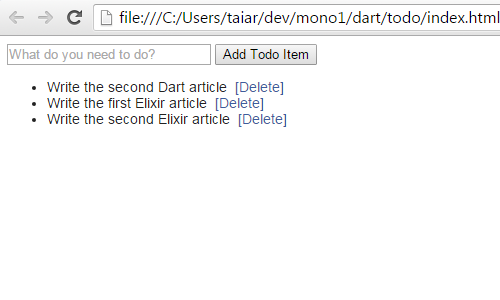
\includegraphics[width=\textwidth]{todo_app.png}
  \caption{Aplicação to-do rodando no browser}
  \label{Rotulo}
\end{figure}

Now I will talk about the usage of the Dart language in this small application.

\subsection{Language structure}

From the very basics, Dart is a class-based, single-inheritance, object-oriented
language with C-style syntax.

The Dart language is also dynamically typed. You can write programs that have no
type annotations whatsoever, and run them, much as you would in JavaScript. One
of the Dart programming language’s most innovative features is the use of
optional types. You may use type annotations in Dart. It will have some
improvements to your program like documentation for humans, documentation for
machines, early error detection (Dart provides a static checker that can warn
you about  potential problems) and sometimes, types can help improve performance
when  compiling to JavaScript.

The static checker acts a lot like in C. It warns you about potential  problems
at compile-time. Many of these warnings are related to types. The static checker
does not produce errors - you can always compile and run your code, no matter
what the checker says.

Let's check out the example:

\begin{lstlisting}[label=dpoint,caption=Dart Warning Example]
class Point {
  final num x, y;
  Point(this.x, this.y);
  Point operator +(Point other) {
    return new Point(x + other.x, y + other.y);
  }

  String toString() {
    return "x: $x, y: $y";
  }
}

main() {
  Point p1 = new Point(0, 0);
  Point p2 = new Point(10, 10);

  int n = p1 + p2;

  print(n);
}
\end{lstlisting}

The code above sends a warning in $int n = p1 + p2;$ saying  $A value of
type 'Point' cannot be assigned to a variable of type 'int'$ if we run the
program with the $checked mode$ turned on. However, the program works nice with
no checking at all.

When no types are provided, Dart avoid complaints by adding a default type
called $dynamic$. We can use this type explicitly:

\begin{lstlisting}[label=dartMap,caption=Dart dynamic type]
Map<String, dynamic> m = {
    'one': new Partridge(),
    'two': new TurtleDove(),
    /* ..., */
    'twelve': new Drummer()};
\end{lstlisting}

Dart has generics too. We can have this kind of list:

\begin{verbatim}
new List<String>();
\end{verbatim}

but you will still be able to write something like

\begin{verbatim}
new List();
\end{verbatim}

and use as a list of $Strings$. The previous example is just a shorthand for

\begin{verbatim}
new List<dynamic>();
\end{verbatim}

The Dart constructor is a method of the class with the same name of the class.
As said before, the protected methods starts with underscore and are not visible
outside the package of the class.

\subsection{Libraries again}

Just like we saw in the language introduction, our program uses external
libraries. The first one is the $dart:html$
library \cite{4_3}. This library manages HTML
elements and other resources for web-based applications that need to interact
with the browser and the DOM (Document Object Model). It includes DOM element
types, CSS styling, local storage, media, speech, events, and more.

The second one is the $dart:indexed_db$
library \cite{4_4}. The IndexedDB is a web
standard for an indexed database which works in the browser. By storing data on
the client in an IndexedDB, a web app gets some advantages, such as faster
performance and persistence. Many browsers supports the use of
IndexedDB \cite{4_5}.In our example, we a using
this database to store the TODO tasks.

The third and last one is the $dart:async$
library \cite{4_6} we saw in the early
examples. In this program, we use $async$ to deal with the events of send
and get data from the HTML5 database (IndexedDB).

In our example, none of these libraries is external to the Dart SDK. So we don't
need to install them with the $pub get$ command. They are all included with a
Dart default installation.

\subsection{Integration with modern browsers (HTML5, IndedexDB and JavaScript API)}

As a language that aims to replace JavaScript on the next years, Dart must have
a strong interoperability with HTML5 elements, browsers functionalities and the
JavaScript existent libraries and apis. Filling the gaps of JavaScript in terms
of functionality is a strategy aligned with Dart purpose to make web app
development more pragmatic.

All of the HTML5 compatibility is implemented in the $dart:html$ library. The
first use of this library we can see in our example is with the function
$querySelector$. This function is like a static method of the library. It finds
the first descendant element of the HTMl document that matches the specified
group of selectors (as parameters of the function) and returns an $Element$
object (that describes a HTML object). The selectors are written in the
form of CSS Selectors \cite{4_7}. JavaScript don't
have a native function to match HTML elements by CSS selectors. This kind of
\"feature missing\" in the JavaScript language brings lots of popularity for some
JavaScript frameworks that aims to fill this kind of gaps in the language. The
most famous of them is jQuery \cite{4_8}
which is so present in JavaScript projects that sometimes is jumbled with the
language itself.

The $Element$ type in Dart \cite{4_9} is an
abstract class, which all HTML elements extend. It implements all HTML browser
behaviors like $events$ as we can see in the snippet:

\begin{verbatim}
querySelector('input#submit').onClick.listen((e) => _onAddTodo());  
\end{verbatim}

The querySelector method matches a Input button Element field with the a ID
attribute equals to \"submit\" and binds to it an event called $onclick$. When
this button is clicked, the private method $_onAddTodo$ is called.

The same patch would be written in vanilla JavaScript in this way:

\begin{lstlisting}[label=jset,caption=Vanilla JavaScript translation]
document.getElementById("submit")
  .addEventListener("click", function(e){
    return _onAddTodo();
  }, false);
\end{lstlisting}

Or even in JavaScript with jQuery this way:

\begin{lstlisting}[label=jjqt,caption=JavaScript with jQuery translation]
$("input#submit").on("click", function(e){
  return _onAddTodo();
});
\end{lstlisting}

The very next browser feature controlled by Dart in the example is the
IndexedDB \cite{4_10} interaction. The Indexed
Database API, or IndexedDB (formerly  WebSimpleDB), is a recommended web browser
standard interface for a local database of records holding simple values and
hierarchical objects. IndexedDB was initially proposed by Oracle in 2009.

The code of the program that open the IndexedDB and return the results is:

\begin{lstlisting}[label=dffexp,caption=Dart open's IndexedDB and return results]
Future open() {
  return window
    .indexedDB
    .open(_TODOS_DB, version: _version, onUpgradeNeeded: _onUpgradeNeeded)
    .then(_onDbOpened)
    .catchError(_onError);
}
\end{lstlisting}

It gets the window of the browser, open the database used by the application,
sets the callback function for when the database is opened and ready to use and
even sets a callback function to deal with errors, all in that lines.

The method that add things on the database is this one:

\begin{lstlisting}[label=dpoint,caption=Dart stores stuff]
Future _addTodo(String text) {
  var trans = _db.transaction(_TODOS_STORE, 'readwrite');
  var store = trans.objectStore(_TODOS_STORE);
  return store.put({
    'text': text,
    'timeStamp': new DateTime.now().millisecondsSinceEpoch.toString()
  }).then((_) => _getAllTodoItems())
  .catchError((e) => _onError);
}
\end{lstlisting}

It opens a transaction \cite{4_11} with the
database, create a object used to store things there and use its method called
put passing the JSON object representing the TODO task to it. Same as before,
the put method is chained with the methods that declares the callbacks for the
function: one for the success and another one for errors.

\subsection{Asynchronous again}

Surely one of the keys concepts to write just about any Dart program is to
understand the asynchronous model as well as the
Future \cite{4_12} and
Stream \cite{4_13} objects.

Very used in our example, a Future is used to represent a potential value, or
error, that will be available at some time in the future. Receivers of a Future
can register callbacks that handle the value or error once it is available.
Those are the callbacks functions I said on the two methods in our previous
topic. A interesting thing is that it applies to the methods that deals with
Input and Output in the program, always heavy operations in any programming
platform.

\chapter{Elixir}
\section{Elixir language introduction}

\subsection{How did it appear?}

Elixir \cite{5_1} is a programming language
designed to build scalable and maintainable systems. It first appeared in may
2012 after 1 year of \textit{underground development} and at first it was a solo
project from its creator and maintainer José
Valim \cite{5_2}. In the begining of 2012,
Plataformatec \cite{5_3}, a brazilian tech company
where José Valim works (and is one of the owners) starts to sponsor and support
the project and then the language got a real improvement.

Even before the first stable version was launched, Elixir attract many
contributors and enthusiasts. It counts 6 written books about programming in
Elixir and other recipes \cite{5_4}, 3
international conferences \cite{5_5} and 300+
open source contributors \cite{5_6}. Besides having
its own community, Elixir is also attracts members of the Ruby and Erlang
communities too.

The version 1.0 of the language \cite{5_7} was
released in September 10 in the year of 2014.

\subsection{Why was it designed and implemented?}

Back in 2010, José Valim was a very active member of the Ruby
Language \cite{5_8} community. He worked on the
core team of a major Ruby open source project called Ruby on
Rails \cite{5_9} (a framework to build web
applications). One of his contributions for this tool was to make the Ruby on
Rails framework **thread safe**. At first, Ruby on Rails applications doesn't
scaled horizontally. At that time, there was no advantage on running a Rails
application on multi-core machines. Making the framework thread safe means that
the application written in Ruby on Rails when deployed in multi-core machines
would run efficiently and use all processing power of that environment and in
the right way (there will exist no problems with concurrency). Valim finds out
that, on that time, there weren't good tools on Ruby ecosystem to work with
concurrency and he started do research about this topics trying to find in other
languages and platforms the best ways to solve the problem they had in Rails.

During his explorations, Valim read the awesome \textbf{7 languages in 7 weeks} 
\cite{5_10} where he meets the Erlang \cite{5_11} programming language. Erlang
is a functional programming language and it has a virtual machine. It was
developed by Ericsson \cite{5_12} and open sourced in 1998. It was designed for
distributed and fault tolerant applications that runs in real time in a
uninterrupted environment.

Very interested in the platform, he started to look deeper in the Erlang
ecossystem writing programs and projects in Erlang. He loved the things the
language has but misses things that he thought to be very important like good
metaprogramming and polimorphysm. Despite these misses, the Erlang Virtual
Machine was really awesome and Erlang was very good in concurrency.

At that time, there was only one language that had all the things Valim wishes
to have in a language and it was Clojure \cite{5_13}.
Clojure is a dynamic language (no statyc typing), very extensible and with great
focus on concurrency. Ruby was a dynamic and extensible language but was not
good in concurrency scenarios like we saw. Go \cite{5_14}
has a focus in concurrency but is static typed and not a very extensible
language. Clojure has all he wants but is a JVM language (language that runs in
the Java Virtual Machine) and he thinks that was a good idea to have other
language option on this niche.

\subsection{How can we use it, e.g., install and run?}

The only prerequisite to run Elixir programs is Erlang 17.0 or later. So, before
install the Elixir you must be sure to have Erlang installed.

\subsubsection{Linux}

There are easy install setups for all major Linux distributions. Most of them
installs the Erlang Virtual Machine too, so yout don't have do care with it. You
can install on Ubuntu based distros with the commands:

\begin{verbatim}
$ wget https://packages.erlang-solutions.com/erlang-solutions_1.0_all.deb && sudo dpkg -i erlang-solutions_1.0_all.deb
$ sudo apt-get update
$ sudo apt-get install elixir
\end{verbatim}

on Red Hat distros with:

\begin{verbatim}
$ yum install elixir
\end{verbatim}

and on Arch Linux with the command:

\begin{verbatim}
$ pacman -S elixir
\end{verbatim}

\subsubsection{Mac OS}

On Mac OS you can install using Homebrew:

\begin{verbatim}
$ brew update
$ brew install elixir
\end{verbatim}

\subsubsection{Windows}

There are precompilled packages for Windows you can download and install on the
Elixir download session at the website. You can also use the Chocolatey tool
and install with:

\begin{verbatim}
cinst elixir
\end{verbatim}

\subsubsection{Testing the installation}

After installing, let's check if we installed right and we can run Elixir
programs in our environment. Elixir code can be scripted and interpreted or
compiled into bytecode that runs on the Erlang VM. Let's checkt the interpreter.

Write and save the following code to the $hello.exs$ file:

\begin{lstlisting}[label=ehw,caption=Elixir Hello World]
IO.puts "Hello, Elixir!"
\end{lstlisting}

and then, run the commands:

\begin{verbatim}
$ elixir hello.exs
\end{verbatim}

and you'll have the $Hello, Elixir!$ sentence on your screen.

For the compilation to bytecodes, the Elixir program must be inside a module.
Write the $hello.ex$ file with the following contents:

\begin{lstlisting}[label=emhw,caption=Elixir Hello World inside a module]
defmodule Hello do
  def say do
    IO.puts "Hello, Elixir!"
  end
end
\end{lstlisting}

and compile with the command:

\begin{verbatim}
$ elixirc hello.ex
\end{verbatim}

Check that the $Elixir.Hello.beam$ file is created with bytecode in the same
directory. Let's check if the module works using the Elixir interactive
environment. Run the program in the command line in this same directory:

\begin{verbatim}
$ iex
Erlang/OTP 18 [erts-7.1] [source] [smp:4:4] [async-threads:10] [kernel-poll:false]

Interactive Elixir (1.1.1) - press Ctrl+C to exit (type h() ENTER for help)
iex(1)>
\end{verbatim}

In the interactive execution environment, type the code:

\begin{verbatim}
iex(1)> Hello.say()
Hello, Elixir!
:ok
\end{verbatim}

and check that it loads the module and executes the function we defined.

\subsection{Simple programs}

Elixir is a functional language (the only functional-only language I learned on
this work). Here are its basic types:

\begin{verbatim}
iex> 1          # integer
iex> 0x1F       # integer
iex> 1.0        # float
iex> true       # boolean
iex> :atom      # atom / symbol
iex> "elixir"   # string
iex> [1, 2, 3]  # list
iex> {1, 2, 3}  # tuple
\end{verbatim}

There are some common features in functional languages that we'll
look on the next examples.

\subsubsection{Anonymous functions}

In the interactive execution environment, let's see some things about anonymous
functions:

\begin{verbatim}
$ iex
Erlang/OTP 18 [erts-7.1] [source] [smp:4:4] [async-threads:10] [kernel-poll:false]

Interactive Elixir (1.1.1) - press Ctrl+C to exit (type h() ENTER for help)
iex(1)> add = fn a, b -> a + b end
#Function<12.54118792/2 in :erl_eval.expr/5>
iex(2)> is_function(add)
true
iex(3)> add
#Function<12.54118792/2 in :erl_eval.expr/5>
iex(4)> add.(2, 4)
6
iex(5)> add_ten = fn a -> add.(a, 10) end
#Function<6.54118792/1 in :erl_eval.expr/5>
iex(6)> add_ten.(11)
21
iex(7)> x = add_ten.(0)
10
iex(8)> x
10
iex(9)> (fn -> x = 42 end).()
42
iex(10)> x
10
\end{verbatim}

Functions are delimited by the keywords **fn** and **end**. They can be assigned
to variables and passed as function parameters just as other types in the
language. In the example, we assing a function that add two variables to a
variable called $add$. To test it, we invoke the anonymous function with $add.$
(we need that point after the variable name to call the anonymous functions) and
then the parameters.

Anonymous functions are clojures and they can access variables that are in scope
when the function is defined, like in the example when we create the $add_ten$
variable. The variable assigned inside a function doesn't affects the outer
scope, so we check it on the last part of the execution.

\subsubsection{Lists, tuples and immutability}

Here are some operations with lists:

\begin{verbatim}
$ iex
Erlang/OTP 18 [erts-7.1] [source] [smp:4:4] [async-threads:10] [kernel-poll:false]

Interactive Elixir (1.1.1) - press Ctrl+C to exit (type h() ENTER for help)
iex(1)> music = [:a, :b, :c] ++ [1, 2, 3]
[:a, :b, :c, 1, 2, 3]
iex(2)> music -- [:c, 3]
[:a, :b, 1, 2]
iex(3)> hd(music)
:a
iex(4)> tl(music)
[:b, :c, 1, 2, 3]
\end{verbatim}

There are the concatenation operator **++** and the subtractor **--** operators
that concatenates and subtract lists and there are the **hd** and **tl**
functions that returns the head and the tail of the list.

\begin{verbatim}
$ iex
Erlang/OTP 18 [erts-7.1] [source] [smp:4:4] [async-threads:10] [kernel-poll:false]

Interactive Elixir (1.1.1) - press Ctrl+C to exit (type h() ENTER for help)
iex(1)> tuple = {:ok, "hello"}
{:ok, "hello"}
iex(2)> put_elem(tuple, 1, "world")
{:ok, "world"}
iex(3)> elem(tuple, 0)
:ok
iex(4)> tuple_size(tuple)
2
iex(5)> elem(tuple, 1)
"hello"
\end{verbatim}

We create a tuple using curly brackets. We can set a value for a determined
tuple position, return a position and get a tuple size. Note in the last command
that the second element of the variable tuple remains the same. The original
tuple stored in the tuple variable was not modified because Elixir data types
are immutable. By being immutable, Elixir code is easier to reason about as you
never need to worry if a particular code is mutating your data structure in
place.

Lists in Elixir are linked. This means that each element in a list holds its
value and points to the following element until the end of the list is reached.
Accessing the length of a list is a linear operation: we need to traverse the
whole list in order to figure out its size. Updating a list is fast as long as
we are prepending elements.

Tuples are stored contiguously in memory. This means getting the tuple size or
accessing an element by index is fast. However, updating or adding elements to
tuples is expensive because it requires copying the whole tuple in memory. Those
performance characteristics dictate the usage of those data structures.

\subsubsection{Pattern matching}

Pattern matching allows to easily destructure data types such as tuples and
lists. It is one of the foundations of recursion in Elixir. Here are some
examples matching lists and tuples.

\begin{verbatim}
$ iex
Erlang/OTP 18 [erts-7.1] [source] [smp:4:4] [async-threads:10] [kernel-poll:false]

Interactive Elixir (1.1.1) - press Ctrl+C to exit (type h() ENTER for help)
iex(1)> {a, b, c} = {:hello, "world", 42}
{:hello, "world", 42}
iex(2)> b
"world"
iex(3)> [a, b, c] = [1, 2, 3]
[1, 2, 3]
iex(4)> b
2
iex(5)> list = [1, 2, 3]
[1, 2, 3]
iex(6)> [0|list]
[0, 1, 2, 3]
iex(7)> [head | tail] = [1, 2, 3]
[1, 2, 3]
iex(8)> head
1
iex(9)> tail
[2, 3]
\end{verbatim}

\subsubsection{Modules}

Elixir groups several functions into modules. In order to create our own modules
we use the **defmodule** macro. We use the **def** macro to define functions in
that module.

\begin{lstlisting}[label=esum,caption=Elixir Module example]
defmodule Math do
  def sum(a, b) do
    a + b
  end
end

Math.sum(1, 2)
\end{lstlisting}

Inside a module, we can define functions with **def** and private functions with
**defp**. A function defined with **def** can be invoked from other modules
while a private function can only be invoked locally.

\begin{lstlisting}[label=econc,caption=Elixir pattern matching and function visibility]
defmodule Concato do

  def concat(a, b) do
    do_concat(a, b)
  end

  defp do_concat([h|t], [a|b]) do
    [h|t] ++ [a|b]
  end

  defp do_concat(a, b) do
    a <> b
  end

end

IO.puts Concato.concat("Merry", "Christmas") #=> MerryChristmas
IO.inspect Concato.concat([:a, :b, :c], [1, 2, 3]) #=> [:a, :b, :c, 1, 2, 3]
\end{lstlisting}

The last example show the usage of a module with two private functions and a
public function. The public function is used for interface with the module and
it calls the possible 2 other functions using pattern matching. When the
arguments are two lists, it calls a function that concatenate lists and when
they are strings, the function that concatenates strings is called.

\subsubsection{Recursion}

Due to immutability, loops in Elixir (as in any functional programming language)
are written differently from imperative languages. Functional languages rely on
recursion: a function is called recursively until a condition is reached that
stops the recursive action from continuing.

\begin{lstlisting}[label=errrr,caption=Elixir recursion]
defmodule Recursion do

  def print_multiple_times(msg, n) when n <= 1 do
    IO.puts msg
  end

  def print_multiple_times(msg, n) do
    IO.puts msg
    print_multiple_times(msg, n - 1)
  end

end

Recursion.print_multiple_times("Gol!", 7)
\end{lstlisting}

Let's use recursion to make some math operations. The example above has three
**public** functions: the first one return the sum of all numbers in the list
and the second return the list with all elements multiplied by two.

\begin{lstlisting}[label=elists,caption=Elixir recursion with lists]
defmodule Math do

  def sum_list([h|t]) do
    sum_list([h|t], 0)
  end

  defp sum_list([head|tail], accumulator) do
    sum_list(tail, head + accumulator)
  end

  defp sum_list([], accumulator) do
    accumulator
  end

  def double_each([head|tail]) do
    [head * 2|double_each(tail)]
  end

  def double_each([]) do
    []
  end

end

IO.puts Math.sum_list([2,3,5]) #=> 10
IO.inspect Math.double_each([2,3,5]) #=> [4, 6, 10]
\end{lstlisting}

Elixir has a Enum \cite{5_15} module that
provides a set of algorithms that enumerate over collections. This module has a
**reduce** and a **map** functions that we'll use to rewrite our last example:

\begin{lstlisting}[label=eenum,caption=Elixir lists with Enum]
defmodule Mathenum do

  def sum_list([h|t]) do
    Enum.reduce([h|t], 0, fn(x, acc) -> x + acc end)
  end

  def double_each([h|t]) do
    Enum.map([h|t], fn(x) -> x * 2 end)
  end

end

IO.puts Mathenum.sum_list([2,3,5]) #=> 10
IO.inspect Mathenum.double_each([2,3,5]) #=> [4, 6, 10]
\end{lstlisting}
\section{Elixir language usage}
On this usage example, we'll use most of the concepts on the last article to 
build a more complex program that explores the concurrent features of Elixir.
Starting with a Fibonacci function we'll increment the program touching concepts
that were not in the first article like pipes, processes, communication between 
processes and tail call optimization.

\subsection{Fibonacci}

Let's begin with a canonical starter recursive Fibonacci implementation with 
Elixir. Here is the code:

\begin{lstlisting}[label=efib1,caption=Classic Fibonacci]
defmodule Fib do

  def fib(0) do 0 end
  def fib(1) do 1 end
  def fib(n) do fib(n - 1) + fib(n - 2) end

end

IO.puts Fib.fib(0)
IO.puts Fib.fib(1)
IO.puts Fib.fib(2)
IO.puts Fib.fib(3)
IO.puts Fib.fib(4)
IO.puts Fib.fib(5)
IO.puts Fib.fib(6)
IO.puts Fib.fib(7)
IO.puts Fib.fib(8)
\end{lstlisting}

Nothing new here, just right to the point. Just write the problem's definition 
and we got the right result:

\begin{verbatim}
  
\end{verbatim}

\begin{verbatim}
$ elixir fib.ex 
0
1
1
2
3
5
8
13
21
\end{verbatim}

\subsection{Many Fibonacci numbers}

Let's improve our last code to generate many numbers passing them as a list to 
the function \cite{6_2}. Here is the code:

\begin{lstlisting}[label=emf,caption=Many Fibonacci numbers]
defmodule Fib do

  def run(list) do
    list
    |> Enum.map(&(fib(&1)))
    |> inspect
    |> IO.puts
  end

  def fib(0) do 0 end
  def fib(1) do 1 end
  def fib(n) do fib(n - 1) + fib(n - 2) end

end

Fib.run([0,1,2,3,4,5,6,7,8])
\end{lstlisting}

The $|>$ symbol used in the snippet above is the pipe operator: it simply 
takes the output from the expression on its left side and passes it as the first
argument to the function call on its right side. It’s similar to the Unix **|** 
operator. Its purpose is to highlight the flow of data being transformed by a 
series of functions. The $run$ function without the pipe operator would be:

\begin{lstlisting}[label=dartMap,caption=Dart dynamic type]
def run(list) do
  IO.puts(inspect(Enum.map(list, fn(x) -> fib(x) end )))
end
\end{lstlisting}

The $Enum.map$ function calls the function on the second parameter for each 
element in the list passed as the first parameter returning a new list with the 
transformed elements. The $inspect$ function returns a String with the list
\"pretty printed\" (written in a human readable format) and we print the list with
the $IO.puts$ function. The result of the execution, for whatever $run$ 
implementations is:

\begin{verbatim}
$ elixir fib.ex 
[0, 1, 1, 2, 3, 5, 8, 13, 21]
\end{verbatim}


\subsection{Parallel Fibonacci numbers}

In our last example, we run the function that calculates each Fibonacci's number
sequentially. The execution waits each of the numbers to be calculated before 
calculate the next number. Running this program for some bigger numbers would be
slow. Let's measure the time to calculate the Fibonacci numbers from 30 to 40:

\begin{verbatim}
$ time elixir fib.ex 
[832040, 1346269, 2178309, 3524578, 5702887, 9227465, 14930352, 24157817, 39088169, 63245986, 102334155]

real  1m2.186s
user  1m1.664s
sys 0m0.684s
\end{verbatim}

Now I'll rewrite the program to calculate these numbers using data parallelism.
Our code will distribute the number calculation across different parallel 
computer cores possibly making the execution faster. Here is the code:

\begin{lstlisting}[label=epf,caption=Parallel processing for Fibonacci in Elixir]
defmodule Fib do

  def run(list) do
    list
    |> Enum.with_index
    |> Enum.map fn(ni) -> spawn_run(self, ni) end
    receive_fibs(length(list), [])
  end

  defp receive_fibs(lns, result) do
    receive do
      fib ->
        result = [fib | result]
        if lns == 1 do
          IO.puts(print_fibs(result))
        else
          receive_fibs(lns - 1, result)
        end
    end
  end

  defp print_fibs(fibs) do
    fibs
    |> Enum.sort(fn({_, a}, {_, b}) -> a < b end)
    |> Enum.map(fn({f, _}) -> f end)
    |> inspect
  end

  def spawn_run(pid, ni) do
    spawn __MODULE__, :send_run, [pid, ni]
  end

  def send_run(pid, {n, i}) do
    send pid, {fib(n), i}
  end

  def fib(0) do 0 end
  def fib(1) do 1 end
  def fib(n) do fib(n - 1) + fib(n - 2) end
end

Fib.run([30,31,32,33,34,35,36,37,38,39,40])
\end{lstlisting}

Our already existent $run$ function was modified. The $Enum.with_index$ 
method returns the collection with each element wrapped in a tuple alongside its
index. This way we can identify this number later to return them in the correct
order. The $Enum.map$ function that used to call the $fib$ function now 
calls a $spawn_run$ function. At the end of the $run$ function it calls a 
$receive_fibs$ function.

The $spawn_run$ function just spawn off new processes \cite{6_1}
of execution. The Elixir's $spawn$ function takes a function which it will 
execute in another process. It returns a PID (process identifier). The spawned 
process will execute the given function and exit after the function is done. The
program uses the $send$ and $receive$ functions to comunicate between 
different proccesses. The $send$ method receives a PID and a message and sends
the message to the proccess with the referred PID. The $receive$ function has 
one parameter that must be a function that will receive the potentially message 
sent. 

So in our code, the $spawn_run$ is called (for each one of the numbers we want
the fibonacci number) and it calls a $send_run$ function. The $send_run$ 
function sends back a result of our already known $fib$ functions. The receive
function is used inside the $receive_fibs$ function. $receive_fibs$ works as
a synchronization function that awaits the execution of all parallel $fib$ 
calls, adding them to a list and returning this list when there is no more 
proccesses running.

When all the execution is over, the $receive$ method calls the $print_fibs$
function. This function orders the calculated number by its index (mentioned on 
the $run$ function). This is necessary because the result of the parallel 
and asynchronous execution times are not deterministic and the order it returns 
the numbers is unknown. At last, the tuples with indexes are removed and just 
the result of the Fibonacci numbers are printed on the screen.

Now, this is the execution time of the parallel version of the program:

\begin{verbatim}
$ time elixir fib.ex 
[832040, 1346269, 2178309, 3524578, 5702887, 9227465, 14930352, 24157817, 39088169, 63245986, 102334155]

real  0m33.141s
user  1m22.564s
sys 0m1.208s
\end{verbatim}

The real execution time of the parallel program is almost the half of the 
execution time for the sequential version of the code. This time would become 
even better if the machine that executes the program has a processor with a 
bigger number of execution cores.

\subsection{Tail call optimization}

Tail-call optimization is where you are able to avoid allocating a new stack 
frame for a function because the calling function will simply return the value 
that it gets from the called function.

The parallel portion of the implementations just remains the same. The 
modification is on the $fib$ functions that now has a tail call, avoiding so 
many recursion calls. Here is the code:

\begin{lstlisting}[label=dartMap,caption=Parallel Fibonacci with tail call optimization]
defmodule Fib do

  def run(list) do
    list
    |> Enum.with_index
    |> Enum.map fn(ni) -> spawn_run(self, ni) end
    receive_fibs(length(list), [])
  end

  defp receive_fibs(lns, result) do
    receive do
      fib ->
        result = [fib | result]
        if lns == 1 do
          IO.puts(print_fibs(result))
        else
          receive_fibs(lns - 1, result)
        end
    end
  end

  defp print_fibs(fibs) do
    fibs
    |> Enum.sort(fn({_, a}, {_, b}) -> a < b end)
    |> Enum.map(fn({f, _}) -> f end)
    |> inspect
  end

  def spawn_run(pid, ni) do
    spawn __MODULE__, :send_run, [pid, ni]
  end

  def send_run(pid, {n, i}) do
    send pid, {fib(n), i}
  end

  def fib(n) do fib(n, 1, 0) end
  def fib(0, _, _) do 0 end
  def fib(1, a, b) do a + b end
  def fib(n, a, b) do fib(n - 1, b, a + b) end

end

Fib.run([30,31,32,33,34,35,36,37,38,39,40])
\end{lstlisting}

It might be more illustrative if shown in a non-functional language, like Python:

\begin{lstlisting}[label=ppppp,caption=Python tail call optimization for Fibonacci]
def fib(i, current = 0, next = 1):
  if i == 0:
    return current
  else:
    return fib(i - 1, next, current + next)
\end{lstlisting}

We can see that now, the real execution time of our program is very smaller than
our two last versions:

\begin{verbatim}
$ time elixir fib.ex 
[832040, 1346269, 2178309, 3524578, 5702887, 9227465, 14930352, 24157817, 39088169, 63245986, 102334155]

real  0m2.321s
user  0m2.152s
sys 0m0.320s
\end{verbatim}


\chapter{Rust}
\section{Rust language introduction}
\subsection{How did it appear?}

Rust  \cite{7_1} is a general-purpose,
multi-paradigm, compiled, systems programming
language. Nowadays, the Rust project is maintained and developed by Mozilla  \cite{7_2}
Research but it starts as a personal project by Mozilla employee Graydon Hoare
 \cite{7_3}  \cite{7_4}.

Graydon starts working on Rust in 2006. He was already a engineer at Mozilla
working on compilers and tools for other languages. He started sketching Rust
thinking in a lot of obvious good ideas, known and loved in other languages,
that haven't made it into widely-used systems languages, or are deployed in
languages that have very poor (unsafe, concurrency-hostile) memory models.

After working long time as a hobby project, he decided to show one such
prototype he'd been working on his spare time to his manager. Mozilla took an
interest and set up a team to work on this language as a component of
longer-term project to rebuild their browser stack around safer, more
concurrent, easier technologies than C++. That larger project is called \"servo\".
Mozilla is funding Rust development because of that.

Mozilla began sponsoring the project in 2009 and announced it in 2010. The
first Rust compiler, that was written in OCaml 
 \cite{7_5}, was dropped and rewritten in a
Rust version that successfully compiled itself in 2011. It is called $rustc$
and uses LLVM  \cite{7_6} as it's back end. The
version 1.0  \cite{7_7} was released in 15 May
2015.

\subsection{Why was it designed and implemented?}

System's programming languages became widely used on the last 50 years since
people started using high-level languages to write operating systems.
Nevertheless, there were always two problems constantly present in this niche:

\begin{itemize}
    \item It's difficult to write secure code (due to the way that languages like C and
          C++ manages memory);
    \item It's hard (but essential) to write multi-threaded concurrent code due to the
          low support the languages of this niche offers to programmers to deal
          with the bugs that writing parallel programs would offer  \cite{7_8}.
\end{itemize}

These are the problems that Rust was made to address. As it's own creator says:

\begin{quotation}
Our target audience is frustrated C++ developers. 
\end{quotation}

on which he includes himself. The performance of safe code (which is one of
things that Rust aims) is expected to be slower than C++, however, the Rust
program's performance is comparable to C++ code that manually implements safer
operations  \cite{7_9}. 

Rust is a compiled, multi-paradigm programming language. It supports
pure-functional, actor-based concurrency, imperative-procedural and
object-oriented programming styles.

\subsection{How can we use it, e.g., install and run?}

\subsubsection{Linux and Mac OS}

Rust has a simple installation proccess on Linux and Mac OS systems. Run the
following line in the command terminal:

\begin{verbatim}
$ curl -sSf https://static.rust-lang.org/rustup.sh | sh
\end{verbatim}

It will download the files, ask for $sudo$ passwords and setup everything
automatically.

\subsubsection{Windows}

There are binaries versions with installers for Windows users at the download
page  \cite{7_10}.

\subsubsection{Testing the installation}

Rust default toolset ships with a build tool called $cargo$
 \cite{7_11}. It is a tool to help manage the
Rust projects. Cargo manages three things: building your code, downloading the
dependencies your code needs, and building those dependencies.

To start a new project with cargo, run the command:

\begin{verbatim}
$ cargo new hello --bin
\end{verbatim}

It will generate the dicrectory called $hello$ with some files on it. On the
directory root it creates a $Cargo.toml$ file with some basic information about
the project and a $src$ directory with a $main.rs$ file on it. This is the
content of the main file:

\begin{lstlisting}[label=rhw,caption=Rust Hello World]
fn main() {
    println!("Hello, world!");
}
\end{lstlisting}

To compile and run the project, in the project's root directory, run the
commands:

\begin{verbatim}
$ cargo build
   Compiling hello v0.1.0 (file:///home/taiar/dev/mono1/rust/hello)
$ cargo run
     Running `target/debug/hello`
Hello, world!
\end{verbatim}

and the hello message just show up. The binary file is located at
$target/debug/hello$ and can be executed directly from the command line
without the cargo tool too.

\begin{verbatim}
$ ./target/debug/hello
Hello, world!
\end{verbatim}

\subsection{Simple programs}

\subsubsection{Primitive types and mutability}

Rust provides access to a wide variety of primitives:

\begin{itemize}
    \item signed integers: $i8$, $i16$, $i32$, $i64$ and $isize$ (pointer size);
    \item unsigned integers: $u8$, $u16$, $u32$, $u64$ and $usize$ (pointer size);
    \item floating point: $f32$, $f64$;
    \item char Unicode scalar values like $'a'$, $\alpha$ and $\infty$ (4 bytes each);
    \item bool either $true$ or $false$;
    \item arrays like $[1, 2, 3]$;
    \item tuples like $(1, true)$.
\end{itemize}

Here are some usage:

\begin{lstlisting}[label=rst,caption=Rust types usage]
fn main() {
    // Variables can be type annotated.
    let logical: bool = true;

    let a_float: f64 = 1.0;  // Regular annotation
    let an_integer   = 5i32; // Suffix annotation

    // Or a default will be used.
    let default_float   = 3.0; // `f64`
    let default_integer = 7;   // `i32`

    let mut mutable = 12; // Mutable `i32`.
}
\end{lstlisting}

Variables in Rust are immutable by default. The program:

\begin{lstlisting}[label=rmtt,caption=Rust mutability mistake]
fn main() {
    let truth = true;
    truth = false;
}
\end{lstlisting}

will result in a compile error:

\begin{verbatim}
error: re-assignment of immutable variable `truth` [E0384]
\end{verbatim}

To be mutable, the variables must explicitly be annotated with $mut$:

\begin{lstlisting}[label=rmutmtu,caption=Rust mutability]
fn main() {
    let mut lie = true;
    lie = false;
}
\end{lstlisting}

The version I'm using is Rust 1.5.0.

\subsubsection{Object oriented programming}

Rust uses $structs$ to create more complex data types \cite{7_12} \cite{7_13}.
For example, if we want to use two numbers to represent a point in the space:

\begin{lstlisting}[label=rstr,caption=Rust structs]
struct Point {
    x: f32,
    y: f32,
}

fn main() {
    let mut point = Point { x: 0, y: 0 };

    point.x = 3;
    point.y = 4;
    
    println!("The point is at ({}, {})", point.x, point.y);
}
\end{lstlisting}

Rust also has the concept of Traits. A trait is a language feature that tells
the Rust compiler about functionality a type must provide. If we want a method
that tells the point distance to the origin:

\begin{lstlisting}[label=rtrait,caption=Rust traits]
use std::f32;

struct Point {
    x: f32,
    y: f32,
}

impl Point {
    fn distanceFromO(&self) -> f32 {
        f32::sqrt(self.x * self.x + self.y * self.y)
    }
}

fn main() {
    let point = Point { x: 3f32, y: 4f32 }; 
    println!("The distance from the origin is ({})", point.distanceFromO(), );
}
\end{lstlisting}

The Trait implements the $distanceFromO$ method for the $Point$ struct.

Visibility in Rust is done around modules. Rust provides a powerful module 
system that can be used to hierarchically split code in logical units (modules),
and manage visibility (public/private) between them. A module is a collection of
items: functions, structs, traits, impl blocks, and even other modules \cite{7_14}.
\section{Rust language usage}
Rust was made to be a system's programming language. There are lots of ways to
integrate Rust programs into computer systems and other programming languages.
In this usage example we'll see how to write a system shared library in Rust and
use it from other programs in other languages.

\subsection{Our problem}

This is the Monte Carlo algorithm for a Pi approximation 
 \cite{8_1} written in Python:

\begin{lstlisting}[label=pytthth,caption=Python Monte Carlo algorithm]
import random
import sys

def montecarlopi(n):
    m = 0.
    n = int(n)
    for i in range(0, n):
        x, y = random.random(), random.random()
        if ((x ** 2) + (y ** 2)) < 1:
            m = m + 1
    return 4 * m / n

print montecarlopi(sys.argv[1])
\end{lstlisting}

It computes a approximation for the Pi value, based in the given parameter. When
bigger is the parameter, better is the approximation value. Let's measure some
executions:

\begin{verbatim}
$ time python pi.py 10
3.6

real    0m0.016s
user    0m0.015s
sys 0m0.000s
\end{verbatim}

The programs is fast and the value is a very bad approximation. Let's increase
the precision:

\begin{verbatim}
$ time python pi.py 100000
3.14184

real    0m0.067s
user    0m0.058s
sys 0m0.008s

$ time python pi.py 1000000
3.140332

real    0m0.533s
user    0m0.504s
sys 0m0.028s

$ time python pi.py 10000000
3.1423776

real    0m5.192s
user    0m4.912s
sys 0m0.276s

$ time python pi.py 100000000
3.14162228

real    3m55.038s
user    0m52.011s
sys 0m6.175s
\end{verbatim}

The program became very slow very fast. It's a common approach to implement the
slow algorithms of the systems in platforms that runs fast and integrate into
the real workflow by calling this solution in other platform. So, let's take a
look on the implementation of this algorithm in Rust:

\begin{lstlisting}[label=rmcalg,caption=Rust Monte Carlo algorithm]
extern crate rand;

use std::env;
use std::str::FromStr;
use rand::distributions::{IndependentSample, Range};

fn montecarlopi(n: u32) -> f32 {
    let between = Range::new(-1f32, 1.);
    let mut rng = rand::thread_rng();

    let total = n;
    let mut in_circle = 0;

    for _ in 0..total {
        let a = between.ind_sample(&mut rng);
        let b = between.ind_sample(&mut rng);
        if a*a + b*b <= 1. {
            in_circle += 1;
        }
    }
    4. * (in_circle as f32) / (total as f32)
}

fn main() {
   let args: Vec<String> = env::args().collect();
   if args.len() > 1 {
     println!("{}", montecarlopi(FromStr::from_str(&args[1]).unwrap()));
   }
}
\end{lstlisting}

It Is the same algorithm at all. Let's measure the execution of this program:

\begin{verbatim}
$ time ./release/point 100000000
3.1413338

real    0m5.323s
user    0m1.911s
sys 0m3.410s

time ./release/point 1000000000
3.1415544

real    0m53.193s
user    0m19.046s
sys 0m34.107s
\end{verbatim}

Awesome! The execution time is much better (even with more precision). Now we
should make it callable from Python and other platforms.

\subsection{A Rust library}

Let's start creating a new project with Cargo:

\begin{verbatim}
$ cargo new montepy
$ cd montepy
\end{verbatim}

Now, edit the ./src/lib.rs file Cargo creates inserting our previous code with
some changes I'll explain later:

\begin{lstlisting}[label=rlllabrar,caption=Rust library code]
extern crate rand;

use std::env;
use std::str::FromStr;
use rand::distributions::{IndependentSample, Range};

#[no_mangle]
pub extern fn montecarlopi(n: u32) -> f32 {
    let between = Range::new(-1f32, 1.);
    let mut rng = rand::thread_rng();

    let total = n;
    let mut in_circle = 0;

    for _ in 0..total {
        let a = between.ind_sample(&mut rng);
        let b = between.ind_sample(&mut rng);
        if a*a + b*b <= 1. {
            in_circle += 1;
        }
    }
    4. * (in_circle as f32) / (total as f32)
}
\end{lstlisting}

The not so odd modification is the $pub extern$ annotations in the font of
the $montecarlopi$ function. The $pub$ means that this function should be
callable from outside of this module, and the $extern$ says that it should be
able to be called from C. Also the $main$ method was removed because we don't
want this program to execute itself. The other modification was the $\#[no_mangle]$ annotation over the method. When you create a Rust library, it
changes the name of the function in the compiled output. This attribute turns
that behavior off  \cite{8_2}.

Also we had to change the $Cargo.toml$ file. It will look like this:

\begin{verbatim}
[package]
name = "montepy"
version = "0.1.0"
authors = ["André Taiar <taiar@dcc.ufmg.br>"]

[dependencies]
rand = "*"

[lib]
name = "montepi"
crate-type = ["dylib"]
\end{verbatim}

The additions here where the $dependencies$ clause, specifying that rand library
is our dependence (Cargo will download and install it for us), the $lib$ clause,
specifying we are building a library and we want to compile our library into a
standard dynamic library  \cite{8_3}. Let's build
the library:

\begin{verbatim}
$ cargo build --release
    Updating registry `https://github.com/rust-lang/crates.io-index`
   Compiling winapi v0.2.5
   Compiling libc v0.2.2
   Compiling winapi-build v0.1.1
   Compiling advapi32-sys v0.1.2
   Compiling rand v0.3.12
   Compiling montepy v0.1.0 (file:///home/taiar/dev/mono1/rust/montepy)
\end{verbatim}

Now in the $./target/release/$ directory there is a file called
$libmontepi.so$ which is our compiled dynamic library. Now, we can create a
python program that uses this library and compute our result very fast. Here is
the code:

\begin{lstlisting}[label=perrr,caption=Python wrong code for calling the library]
from ctypes import cdll

lib = cdll.LoadLibrary("target/release/libmontepi.so")
print lib.montecarlopi(100000000)

print("done!")
\end{lstlisting}

The execution result:

\begin{verbatim}
$ time python pi.py 
22862944
done!

real    0m5.412s
user    0m2.061s
sys 0m3.343s
\end{verbatim}

The program runs really fast but wait, there is a problem. The aproximation
result is totally wrong.

The problem is that the integers and floats we use in our implementation of the
Rust algorithm has different forms from the types of Python. To get around this,
we must convert our numbers for types that are compatible with our system. Here
is our new Python code:

\begin{lstlisting}[label=pytonright,caption=Python right code]
from ctypes import cdll
import ctypes

lib = cdll.LoadLibrary("target/release/libmontepi.so")

montecarlopi = lib.montecarlopi
montecarlopi.restype = ctypes.c_float
print montecarlopi(100000000)

print("done!")
\end{lstlisting}

\begin{verbatim}
$ time python pi.py 
3.14137887955
done!

real  0m5.400s
user  0m1.952s
sys 0m3.447s
\end{verbatim}

and in Node.js (with the ffi package  \cite{8_4}):

\begin{lstlisting}[label=njs,caption=Node calling our Rust library]
var ffi = require('ffi');

var pipi = ffi.Library('./target/release/libmontepi.so', {
    'montecarlopi': ['float', ['int']]
});

console.log(pipi.montecarlopi(100000000));
\end{lstlisting}

\begin{verbatim}
$ time nodejs pi.js 
3.1415293216705322

real  0m5.466s
user  0m2.038s
sys 0m3.420s
\end{verbatim}

and in C (the $libmontepi.so$ file must be available in your system):

\begin{lstlisting}[label=ccorl,caption=C calling our Rust library]
#include <stdint.h>
#include <stdio.h>

float montecarlopi(const int precision);

int main() {
  printf("%f\n", montecarlopi(100000000));
  return 0;
}
\end{lstlisting}

\begin{verbatim}
$ gcc -o pi pi.c -lmontepi
$ time ./pi 
3.141783

real  0m5.367s
user  0m1.925s
sys 0m3.441s
\end{verbatim}


\bibliography{bibliog}

\end{document}
